\documentclass[11pt]{article}
\usepackage[margin=1in]{geometry}
\usepackage{amsmath,amssymb,amsthm,mathtools}
\usepackage{graphicx}
\usepackage[hidelinks]{hyperref}
\usepackage{xcolor}

\newtheorem{theorem}{Theorem}
\newtheorem{remark}[theorem]{Remark}
\newcommand{\R}{\mathbb R}
\setlength{\emergencystretch}{2em}

\title{Right Haar measure on the affine group refutes\\
the Modular Collapse Conjecture}
\author{Autonomous mathematical discovery run \texttt{fa\_banach\_001}}
\date{27 August 2026}

\begin{document}
\maketitle

\noindent\textbf{Status.}
Candidate full negative answer, likely valid pending expert review.

\section{Source conjecture}

Inou\'e defines a left quasi-invariant measure on a locally compact
topological quasigroup $Q$ to be a nonzero regular Borel measure $\mu$ for
which
\[
 (L_a)_*\mu=j(a)\mu \qquad (a\in Q)
\]
with positive scalar cocycle $j$.  Conjecture~1, the \emph{Modular Collapse
Conjecture}, asserts that if $Q$ satisfies
\[
 ((xy)z)y=x(y(zy)) \tag{N1}
\]
and admits such a measure, then $j\equiv1$
\cite[Conjecture~1, PDF p.~16]{Inoue}.

\begin{center}
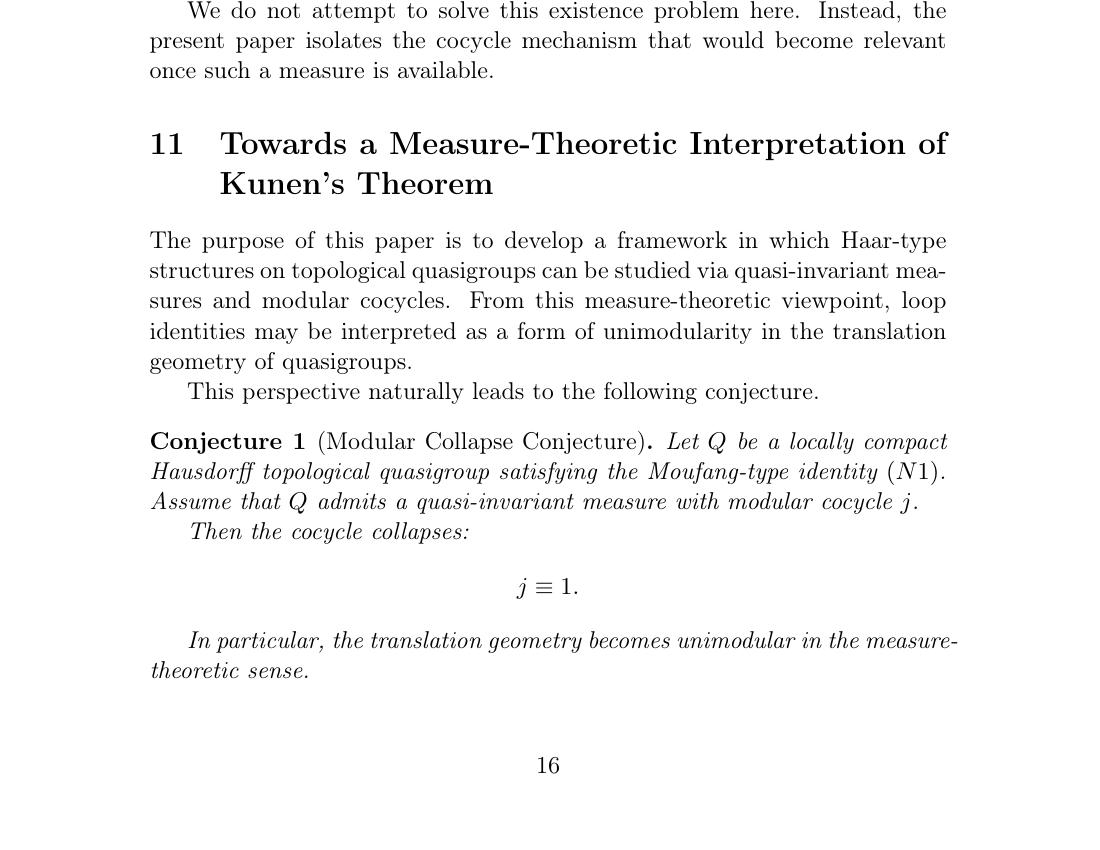
\includegraphics[width=0.68\textwidth]{figures/open_conjecture.png}
\end{center}

We give a counterexample which satisfies the stronger, two-sided
quasi-invariance hypothesis used elsewhere in the source.

\section{Counterexample}

\begin{theorem}\label{thm:main}
The Modular Collapse Conjecture is false.  In fact, there is a connected
two-dimensional Lie group $G$, regarded as a topological quasigroup, and a
nonzero regular Borel measure $\nu$ such that
\[
 (L_g)_*\nu=j(g)\nu,\qquad (R_g)_*\nu=\nu
 \quad(g\in G),
\]
but $j\not\equiv1$.
\end{theorem}

\begin{proof}
Let
\[
 G=\{(a,b):a>0,\ b\in\R\},
 \qquad
 (a,b)(a',b')=(aa',\,b+ab').
\]
This is the group of orientation-preserving affine transformations of the
line.  It is a locally compact Hausdorff topological group and hence a
topological quasigroup.  Associativity gives, for every $x,y,z\in G$,
\[
 ((xy)z)y=xyzy=x(y(zy)),
\]
so $(N1)$ holds.

On the open half-plane $G\subset\R^2$, define
\[
 d\nu(a,b)=\frac{da\,db}{a}.
\]
The density is positive and continuous, so $\nu$ is a nonzero regular Borel
measure, finite on compact sets.

Fix $g=(\alpha,\beta)\in G$.  Left translation is
\[
 L_g(a,b)=(\alpha a,\,\beta+\alpha b).
\]
With
\[
 u=\alpha a,\qquad v=\beta+\alpha b,
\]
we have $du\,dv=\alpha^2da\,db$ and $a=u/\alpha$.  Therefore, for every
nonnegative Borel function $f$,
\begin{align*}
 \int_G f\,d((L_g)_*\nu)
 &=\int_G f(\alpha a,\beta+\alpha b)\frac{da\,db}{a}\\
 &=\frac1\alpha\int_G f(u,v)\frac{du\,dv}{u}.
\end{align*}
Thus
\[
 (L_{(\alpha,\beta)})_*\nu=\alpha^{-1}\nu,
 \qquad j(\alpha,\beta)=\alpha^{-1}.
\]

For completeness, right translation is
\[
 R_g(a,b)=(a\alpha,\,b+a\beta).
\]
Now $u=a\alpha$, $v=b+a\beta$, so $du\,dv=\alpha,da\,db$ and again
$a=u/\alpha$.  Hence
\begin{align*}
 \int_G f\,d((R_g)_*\nu)
 &=\int_G f(a\alpha,b+a\beta)\frac{da\,db}{a}\\
 &=\int_G f(u,v)\frac{du\,dv}{u}.
\end{align*}
Consequently $(R_g)_*\nu=\nu$: the chosen measure is right Haar and is
two-sided quasi-invariant in the source's scalar sense.

All hypotheses of Conjecture~1 hold, while
\[
 j(2,0)=\frac12\ne1.
\]
This refutes the conjecture.
\end{proof}

\section{Structural diagnosis}

The source correctly derives multiplicativity of $j$ under $(N1)$ and
two-sided quasi-invariance.  The example above obeys that conclusion:
\[
 j\bigl((a,b)(a',b')\bigr)=(aa')^{-1}
 =j(a,b)j(a',b').
\]
What fails is the extra step from multiplicativity to triviality.  Loop or
group structure normalizes $j$ at the identity but does not eliminate
nontrivial positive characters.  Indeed, the source explicitly notes this
possibility before stating the conjecture.

The counterexample is not sensitive to the one-sided wording of the
conjecture: $\nu$ is invariant under every right translation.  The same
mechanism works for any non-unimodular locally compact group after choosing
right rather than left Haar measure.

\section{Scope, verification, and novelty}

The theorem gives a full negative answer to Conjecture~1 as written.  It does
not classify additional hypotheses that force modular collapse.  Requiring
the chosen measure itself to be left invariant forces $j=1$ by definition;
finding non-tautological rigidity assumptions is a separate question.

The accompanying exact SymPy script verifies both Jacobian-density factors,
the identity $(N1)$ in affine coordinates, and multiplicativity of $j$.  It is
a regression check and is not needed for the proof.

A bounded novelty search on 27 August 2026 covered the four run indexes, the
current arXiv record, the exact conjecture name, the paper title, and variants
combining the affine group, right Haar measure, and the modular cocycle.  No
later answer was found.  The affine-group Haar formulas are standard; the
claimed contribution is their direct application to the new conjecture.
Novelty confidence is moderate pending specialist review.

\paragraph{Human review recommendation.}
Check the source's push-forward convention and the two changes of variables.
Also confirm that “a quasi-invariant measure” in Conjecture~1 has the literal
meaning of the paper's definition rather than an unstated left-Haar
normalization.

\begin{thebibliography}{9}
\raggedright
\bibitem{Inoue}
T. Inou\'e,
\emph{Haar-Type Measures on Topological Quasigroups and Kunen's Theorem},
arXiv:2603.06174v2 (2026).
\end{thebibliography}

\end{document}
